%Master File:lectures.tex

\lesson{Ensemble Methods}
\vspace{-1cm}
\begin{center}
  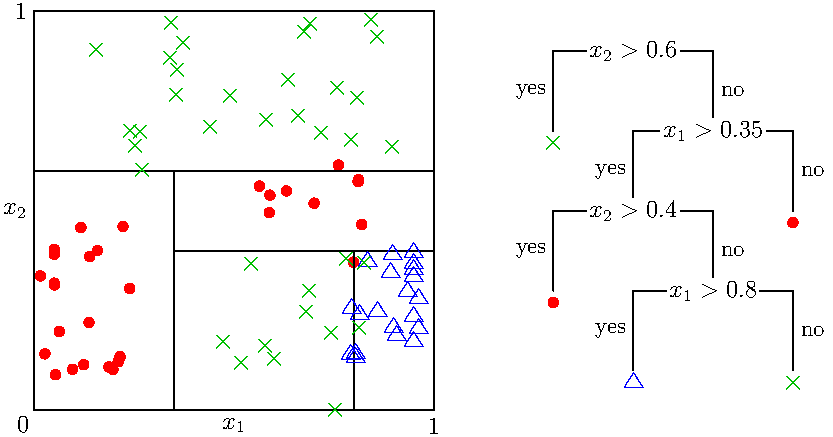
\includegraphics[height=12cm]{decisionTree-5}
\end{center}

\keywords{Decision Trees, Averaging, Bagging}


%%%%%%%%%%%%%%%%%%%%%%% Next Slide %%%%%%%%%%%%%%%%%%%%%%%
\renewcommand{\Outline}{%
\begin{slide}
\section[1]{Outline}

\begin{minipage}{8cm}\raggedright
  \begin{enumerate}
    \outlineitem{Decision Trees}{decisiontreees}
    \outlineitem{Bagging}{bagging}
  \end{enumerate}
\end{minipage}\hfill
\begin{minipage}{15cm}
  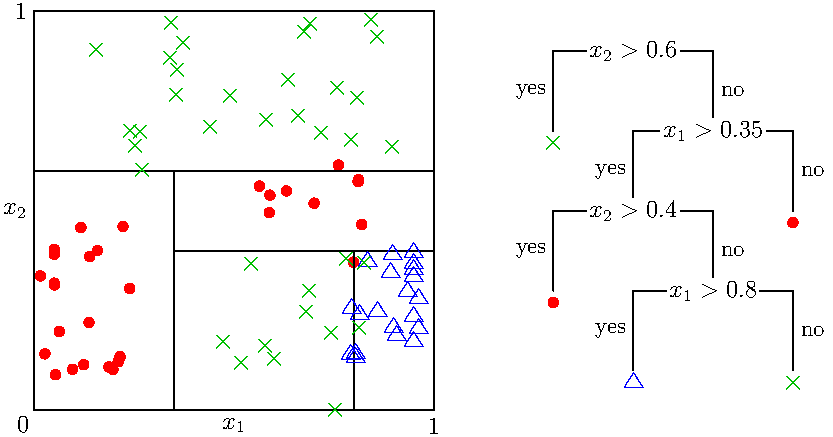
\includegraphics[width=15cm]{decisionTree-5}
\end{minipage}
\end{slide}
\addtocounter{outlineitem}{1}
}

\setcounter{outlineitem}{1}

%%%%%%%%%%%%%%%%%%%%%%% Next Slide %%%%%%%%%%%%%%%%%%%%%%%
\Outline %  Ensemsble Learning
\toptarget{firstoutline}
%%%%%%%%%%%%%%%%%%%%%%% Next Slide %%%%%%%%%%%%%%%%%%%%%%%

\begin{slide}
\section{Removing Variance By Averaging}

\begin{PauseHighLight}
  \begin{itemize}
  \item We can reduce the variance and hence improve our generalisation
    error by averaging over different learning machines\pause
  \item There are a number of different techniques for doing this that
    go by the name of \emph{ensemble methods} or \emph{ensemble
      learning}\pause
  \item This trick can be used with many different learning machines,
    but is clearly most practical for machine that can be trained
    quickly\pause
  \item (nevertheless, even for deep learning taking the average
    response of many machines is usually done to win competitions)\pauseb
  \end{itemize}
\end{PauseHighLight}

\end{slide}

%%%%%%%%%%%%%%%%%%%%%%% Next Slide %%%%%%%%%%%%%%%%%%%%%%%

\begin{slide}
\section{Ensembling of Decision Trees}

\begin{PauseHighLight}
  \begin{itemize}
  \item One set of algorithms where ensembling are common place are
    decision trees\pause
  \item These are particularly good for handling messy data
    \begin{itemize}
    \item categorical data\pause
    \item mixture of data types\pause
    \item missing data\pause
    \item large data sets\pause
    \item multiclass\pause
    \end{itemize}
  \item In many competitions ensembled trees, particularly
    \textit{random forests} and \textit{gradient boosting} beat all
    other techniques\pause
  \end{itemize}
\end{PauseHighLight}

\end{slide}

%%%%%%%%%%%%%%%%%%%%%%% Next Slide %%%%%%%%%%%%%%%%%%%%%%%

\begin{slide}
\section{Decision Trees}

\begin{PauseHighLight}
  \begin{itemize}
  \item A decision trees builds a binary tree to partition the data,
    $\mathcal{D}=\{(\bm{x}_i, y_i)|i=1,\ldots,m\}$, into the leaves of
    the tree\pause
  \item Each decision rule depends on a single feature\pause
  \item At each step the rule is chosen that maximise the
    ``\textit{purity}'' of the leaf nodes\pause
  \item Decisions can be made on numerical values or categories\pause
  \end{itemize}
\end{PauseHighLight}

\end{slide}

%%%%%%%%%%%%%%%%%%%%%%% Next Slide %%%%%%%%%%%%%%%%%%%%%%%

\begin{slide}
\section[-2]{Partitioning}

\begin{PauseHighLight}
  \begin{itemize}
  \item Consider a classification problems with examples $(\bm{x}, y)$
    belonging to some classes $y\in\mathcal{C}$\pause
  \item The data is partitioned by the tree into leaves
    \begin{center}
      \includegraphics[width=0.62\linewidth]{treePicture}\pause
    \end{center}
    \vspace*{-1.6em}

  \item The proportion of data points in leaf $\mathcal{L}$ belonging to
    class $c$ is
    \begin{align*}
      p_{c}(\mathcal{L}) = \frac{1}{|\mathcal{L}|}
      \sum_{(\bm{x},y)\in\mathcal{L}} \pred{y = c}
    \end{align*}
    where $\pred{y = c} = 1$ if $y=c$ and 0 otherwise\pause
  \end{itemize}
\end{PauseHighLight}

\end{slide}

%%%%%%%%%%%%%%%%%%%%%%% Next Slide %%%%%%%%%%%%%%%%%%%%%%%

\begin{slide}
\section[-1]{Leaf Purity}

\begin{PauseHighLight}
  \begin{itemize}
  \item Two different purity measures, $Q_m(\mathcal{L})$, for a leaf node
    $\mathcal{L}$ are commonly used\pause
    \begin{itemize}
    \item \emph{Gini index}
      
      \begin{rightImage}{gini}
        \begin{align*}
          Q^g_m(\mathcal{L}) = \sum_{c\in\mathcal{C}} p_{c}(\mathcal{L})\,
          \left(1-p_{c}(\mathcal{L})\right)\pause
        \end{align*}
      \end{rightImage}
    \item \emph{Cross-entropy}
      
      \begin{rightImage}{crossEnt}
        \begin{align*}
          Q^e_m(\mathcal{L}) = - \sum_{c\in\mathcal{C}} p_{c}(\mathcal{L})\,
          \logg{p_{c}(\mathcal{L})} \pause        
        \end{align*}
      \end{rightImage}
    \end{itemize}
  \end{itemize}
\end{PauseHighLight}

\end{slide}


%%%%%%%%%%%%%%%%%%%%%%% Next Slide %%%%%%%%%%%%%%%%%%%%%%%

\begin{slide}
\section[-1]{Building Decision Trees}

\pb\pause\pauselevel{=1}
\begin{center}
  \multipdf[width=\linewidth]{decisionTree}\pause
\end{center}

\end{slide}

%%%%%%%%%%%%%%%%%%%%%%% Next Slide %%%%%%%%%%%%%%%%%%%%%%%

\begin{slide}
\section{Observations}

\begin{PauseHighLight}
  \begin{itemize}
  \item Decision trees are very useful for exploring new data
    sets\pause---the tree shows what features are most
    important\pause
  \item Decision trees can also be used for regression problems\pause
    \begin{itemize}
    \item Approximate function by a series of rules\pause
    \item Reduce variance between data points assigned to leaf
      nodes\pause
    \end{itemize}
  \item CART is a classic implementation that builds
    \emph{C}lassification \emph{A}nd \emph{R}egression
    \emph{T}rees\pause
  \item Decision trees depend strongly on the early decisions and so
    vary a lot for slightly different data sets\pause---high variance\pauseb
  \end{itemize}
\end{PauseHighLight}

\end{slide}

%%%%%%%%%%%%%%%%%%%%%%% Next Slide %%%%%%%%%%%%%%%%%%%%%%%
\Outline %  Bagging
%%%%%%%%%%%%%%%%%%%%%%% Next Slide %%%%%%%%%%%%%%%%%%%%%%%


\begin{slide}
  \section[-2]{Error In The Means}
  \pb
  \begin{itemize}
  \item By taking the mean over many samples we can reduce the
    variance and thus improve our generalisation performance\pauseh
  \item To get a feel for this consider estimating the mean of a
    random variable, $X$, from a number of samples ($n=5$ in the
    example below)\pauseh    
  \end{itemize}
    \begin{center}
      \multipdf[width=\linewidth]{standardError}\pause
    \end{center}
\end{slide}

%%%%%%%%%%%%%%%%%%%%%%% Next Slide %%%%%%%%%%%%%%%%%%%%%%%

\begin{slide}
\section[-2]{Mean and Variance}

\begin{PauseHighLight}\small
  \begin{itemize}
  \item The expected value of the mean, $\hat{\mu}_n$, of $n$ random
    \emph{independent} variables, $X_i$, is the expected value $\mu=\av{X_i}$
    \begin{align*}
      \av{\hat{\mu}_n}
      =\av{\frac{1}{n} \sum_{i=1}^n X_i } = \frac{1}{n} \sum_{i=1}^n
      \av{X_i} \pause = \frac{1}{n} \sum_{i=1}^n \mu = \mu\pause
    \end{align*}
  \item The variance is $\av{ (\hat{\mu}_n-\mu)^2 }$ or equivalently 
    \begin{align*}
      \frac{1}{n^2} \, \av{ \left(\sum_{i=1}^n (X_i -\mu)\right)^2}
      &=\frac{1}{n^2} \, \av{ \sum_{i=1}^n (X_i -\mu)^2
        + \sum_{i=1}^n\sum_{j=1\atop j\neq i}^n (X_i-\mu)\,(X_j-\mu)}\pause\\
      &= \frac{1}{n^2}\sum_{i=1}^n \left( \av{(X_i -\mu)^2}
        + \sum_{j=1\atop j\neq i}^n
      \av{X_i-\mu}\,\av{X_j-\mu} \right)\pause\\
      &=\frac{1}{n^2} \sum_{i=1}^n \sigma^2\pause = \frac{1}{n} \sigma^2
        \pause
    \end{align*}
  \end{itemize}
\end{PauseHighLight}


\end{slide}

%%%%%%%%%%%%%%%%%%%%%%% Next Slide %%%%%%%%%%%%%%%%%%%%%%%

\begin{slide}
\section[-2]{Bootstrap Aggregation (Bagging)}

\pb
\begin{itemize}
\item To reduce the variance in a learning machine (such as a decision
  tree) we can average over many machines\pauseh
\item To average many machines they must learn something different\pauseh
\item We only have one data set, but we can resample from the data set
  to make them look a bit different\pauseh---this is known a
  \emph{bootstrapping}\pauseh
\end{itemize}
\begin{center}
  \multipdf[width=\linewidth]{bootstrapping}\pause
\end{center}

\end{slide}

%%%%%%%%%%%%%%%%%%%%%%% Next Slide %%%%%%%%%%%%%%%%%%%%%%%

\begin{slide}
\section{Performance of Bagging}

\begin{PauseHighLight}
  \begin{itemize}
  \item For classification we get our different machines to vote\pause
  \item For regression we can average the prediction of different
    machines\pause
  \item Bagging improves the performance of decision trees\pause
  \item However, we can usually do better using Boosting\pause
  \item This is because our decision trees are correlated\pause
  \end{itemize}
\end{PauseHighLight}

\end{slide}


%%%%%%%%%%%%%%%%%%%%%%% Next Slide %%%%%%%%%%%%%%%%%%%%%%%

\begin{slide}
\section{Variance of Positive Correlated Variables}

\begin{PauseHighLight}
  \begin{itemize}
  \item If we calculate the variance of the mean of positively correlated
    variables with correlation $\rho$ we find
    \begin{align*}
      \frac{1}{n^2} \, \av{ \left(\sum_{i=1}^n X_i -\mu\right)^2}
      &= \rho\,\sigma^2 + \frac{1-\rho}{n} \sigma^2
    \end{align*}
  ($\rho = \av{(X_i-\mu)\,(X_j-\mu)}/\sigma^2$)\pause
  \item As $n\rightarrow\infty$ the second term vanishes, but we are left
    with the first term\pause
  \item If we want to do well we need our learning machines to be
    unbiased and decorrelated\pause
  \end{itemize}
\end{PauseHighLight}


\end{slide}


%%%%%%%%%%%%%%%%%%%%%%%xt Slide %%%%%%%%%%%%%%%%%%%%%%%

\begin{slide}
\section{Random Forest}

\begin{PauseHighLight}
  \begin{itemize}
  \item In random forests we average much less correlated trees\pause
  \item To do this for each tree we choose a subset of $p'\ll p$ of the
    features on which to split the tree\pause
  \item Typically $p'$ can range from 1 to $\sqrt{p}$\pause
  \item The trees aren't that good, but are very decorrelated\pause
  \item By averaging over a huge number of trees (order of 1000) we
    typically get good results\pause
  \item Random Forest won (wins?) many competitions\pause
  \end{itemize}
\end{PauseHighLight}

\end{slide}


\begin{slide}
\section{Lessons}

\begin{PauseHighLight}
  \begin{itemize}
  \item Ensemble methods have proved themselves to be very
    powerful\pause
  \item They work by averaging over different machines, trying to
    reduce their variance\pause
  \item Here the variance comes from forcing the machines to learn
    different functions using Bootstrap Aggregation\pause
  \item Tend to work best with very simple models (true of random forest
    and boosting)\pause---seems to reduce over-fitting\pause
  \item Random forest is very powerful, but gradient boosting is competitive\pause
  \end{itemize}
\end{PauseHighLight}

\end{slide}


%%% Local Variables:
%%% TeX-master: "lectures"
%%% End:
